%%%%%%%%%%%%%%%%%%%%%%%%%%%%%%%%%%%%%%%%%%%%%%%%%%%%%%%%%%%%%%%%%%%%%%%%%%%%%%%
\subsection{Introduction to Supervised Learning}
\label{subsection:ch2-introduction_on_supervised_learning}
%%%%%%%%%%%%%%%%%%%%%%%%%%%%%%%%%%%%%%%%%%%%%%%%%%%%%%%%%%%%%%%%%%%%%%%%%%%%%%%

Supervised learning consists in learning a function that maps an input to an output based on input-output pairs.
For example, one could learn to ``predict'' if a fruit will be tasty based on its features (\eg, size, weight, color, consistency, etc.).
These features are used as inputs to the function and the function outputs a value characterizing the taste of the fruit.

In the following, we will formalize the learning problem described above with the \emph{statistical learning framework}.
First, let us define the domain space $\Xset$ which corresponds to the set of inputs that we wish to label.
Let us denote the label space $\Yset$ and a finite sequence of pairs $\Sset = \left\{ \left(\xvec^{(1)}, y^{(1)} \right) \dots \left( \xvec^{(m)}, y^{(m)} \right) \right\}$ in $\Xset \times \Yset$.
Such pairs \ie, labeled examples, are called \emph{training examples} and the set $\Sset$ is called the \emph{training set}.
We denote $\Dset$ the \emph{joint distribution} over $\Xset \times \Yset$.
The main objective of the task at hand is to output a function $h: \Xset \rightarrow \Yset$ that maps the input $\xvec \in \Xset$ to the output $y \in \Yset$.
This function is called the \emph{hypothesis} or the \emph{classifier}.
Given the probability distribution $\Dset$, we aim to measure how \emph{likely} the hypothesis $h$ makes an error when labeled points are randomly drawn from the distribution $\Dset$.
Let us define the true error or \emph{risk} of the hypothesis $h$ that we wish to minimize:
\begin{equation} \label{equation:ch2-risk}
  R_{\Dset}(h) \triangleq \Ebb_{(\xvec, y) \sim \Dset} \left[ L\big( h(\xvec), y \big) \right] \enspace.
\end{equation}
where $L: \Yset \times \Yset \rightarrow \Rbb_{+}$ is a \emph{loss function} which measures the correctness of the hypothesis.
For example, for classification problems, we can use the 0-1 loss defined as: %$L(h(\xvec), y) = \mathds{1}_\big[ h(\xvec) \neq y \big]$.
\begin{equation}
  L(h(\xvec), y) \triangleq \mathds{1}_{\big[ h(\xvec) \neq y \big]}
\end{equation}

However, in practice, the joint probability distribution $\Dset$ is unknown; therefore, the true error is not directly available to the learner.
The learner only has access to the training data, $\Sset$, and can calculate the \emph{empirical error} \ie, the error over the training samples.
We define the \emph{empirical risk} as follows:
\begin{equation} \label{equation:ch2-empirical_risk}
  R_{\Sset}(h) \triangleq \frac{1}{|\Sset|} \sum_{(\xvec, y) \in \Sset} L\big( h(\xvec), y \big) \enspace.
\end{equation}
The learning paradigm which consists in minimizing this value is called \emph{Empirical Risk Minimization} denoted ERM.



% \begin{equation}
%   R_{\Sset}(h) \triangleq \frac{\left| \left\{i \in [m]: h\left(\xvec^{(i)}\right) \neq y^{(i)} \right\}\right|}{m} \enspace.
% \end{equation}
% We can generalize our measure of correctness so that it can be applied to multiple learning tasks.
% Let us define a \emph{loss function} from $\Yset \times \Yset$ to the set of nonnegative real numbers, $L: \Yset \times \Yset \rightarrow \Rbb_{+}$.
% We can express the \emph{risk} as follows:
% \begin{equation}
%   R_{\Dset}(h) \triangleq \Ebb_{(\xvec, y) \sim \Dset} \left[ L\big( h(\xvec), y \big) \right] \enspace.
%   \label{equation:ch2-risk}
% \end{equation}
% Similarly, we express the empirical risk as follows:
% \begin{equation}
%   R_{\Sset}(h) \triangleq \frac{1}{m} \sum_{(\xvec, y) \sim \Sset} L\big( h(\xvec), y \big) \enspace.
% \end{equation}
% The loss functions used for classification problems and regression problems are as follows: 
% \begin{itemize}
%   \item \textbf{0-1 Loss}: $L_{0-1}\big( h(\xvec), y \big) = \mathds{1}_\big[ h(\xvec) \neq y \big]$ \\
%   This loss is used for classification problems, for example, when the learner have to recognizing hand-written digits in images.
%   We can notice that the definitions of $R_{\Dset}$ given in \Cref{equation:ch2-risk1} and \Cref{equation:ch2-risk2} coincide.
%   \item \textbf{Square Loss}: $L_{\text{sq}} \big( h(\xvec), y \big) = \big( h(\xvec) - y \big)^2$ \\	
%   This loss is used for another common type of learning problem \ie, \emph{regression problem}, in which the label domain $\Yset$ is the set of real numbers.
%   For example, one wishes to predict the price of an apartment given its characteristics.
% \end{itemize}


% The goal of the learning algorithm is to find the hypothesis $h$ that minimizes the risk $R_{\Sset}$, this learning paradigm is called \emph{Empirical Risk Minimization} (ERM).
We use the ERM paradigm as a surrogate to find a hypothesis $h$ that minimizes the true risk $R_\Dset$.
However, all hypotheses that minimize the empirical error do not necessarily minimize the true risk.
For example, consider the following function:
\begin{equation} \label{equation:ch2-perfect_function}
  h_c(\xvec) =
  \begin{cases}
    y^{(i)} &\quad \text{if }\exists i \in [m] \text{ s.t. } \xvec^{(i)} = \xvec \\
    c &\quad \text{otherwise}
  \end{cases}
\end{equation}
Clearly, this function, for any training set, $\Sset$, will have $R_\Sset(h_1) = R_\Sset(h_2) = 0$, whereas one the two functions will have a true risk $\geq \frac{1}{2}$ (under the reasonable assumption that $\Sset$ is a negligible set with respect to $\Dset$).
The phenomenon, called \emph{overfitting}, happens when the classifier fits the training data ``too well'' but will likely have a high error on unseen data.
One possible solution to this phenomenon is to apply ERM with a restricted search space to prevent the learning algorithm to output a function such as $h_c$ in \Cref{equation:ch2-perfect_function}.
We call this set the \emph{hypothesis class} and is denoted $\Hset$.
Each $h \in \Hset$ is a function mapping from $\Xset$ to $\Yset$.
We call $\mathrm{ERM}_{\Hset}$, the set of learned hypotheses that uses the $\mathrm{ERM}$ paradigm over the hypothesis class $\Hset$ and a training data $\Sset$.
Formally,
\begin{equation}
  \mathrm{ERM}_{\Hset}(\Sset) = \argmin_{h \in \Hset} R_{\Sset}(h) \enspace.
\end{equation}


\begin{figure}[t]
  \centering
  \begin{subfigure}[b]{0.32\textwidth}
    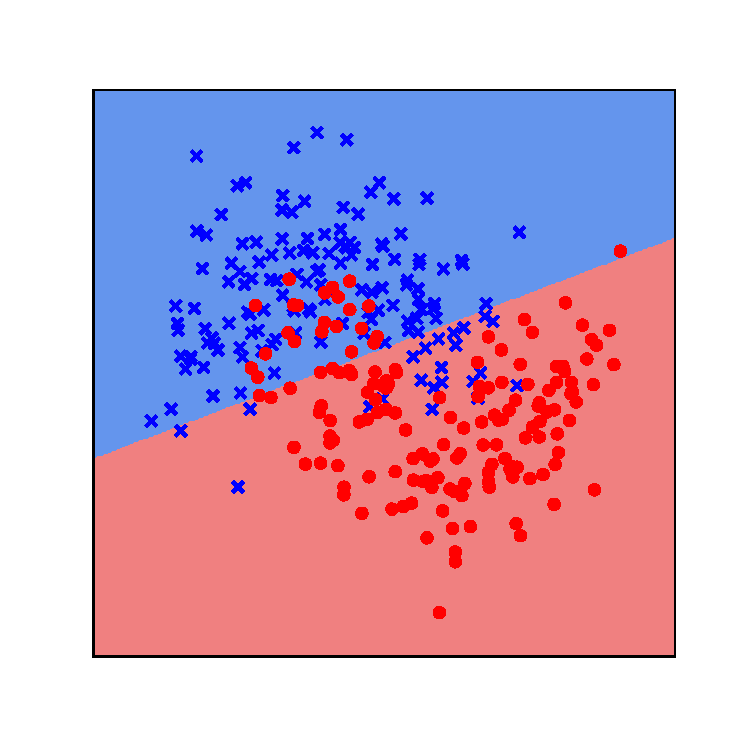
\includegraphics[width=0.98\textwidth]{figures/main/ch2-background/underfitting.pdf}
    \caption{Underfitting}
    \label{figure:ch2-fitting_points_a}
  \end{subfigure}
  \hfill
  \begin{subfigure}[b]{0.32\textwidth}
    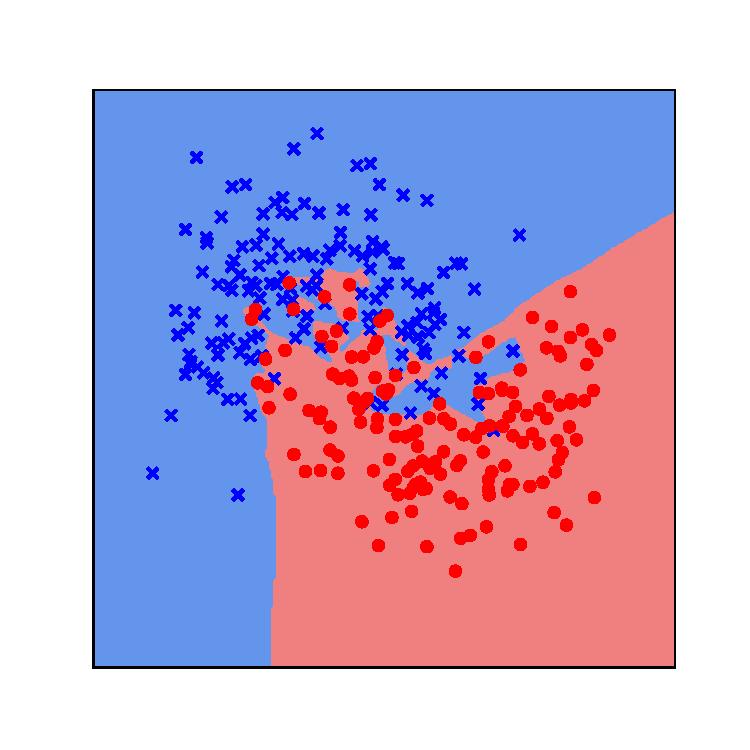
\includegraphics[width=0.98\textwidth]{figures/main/ch2-background/overfitting.pdf}
    \caption{Overfitting}
    \label{figure:ch2-fitting_points_b}
  \end{subfigure}
  \hfill
  \begin{subfigure}[b]{0.32\textwidth}
    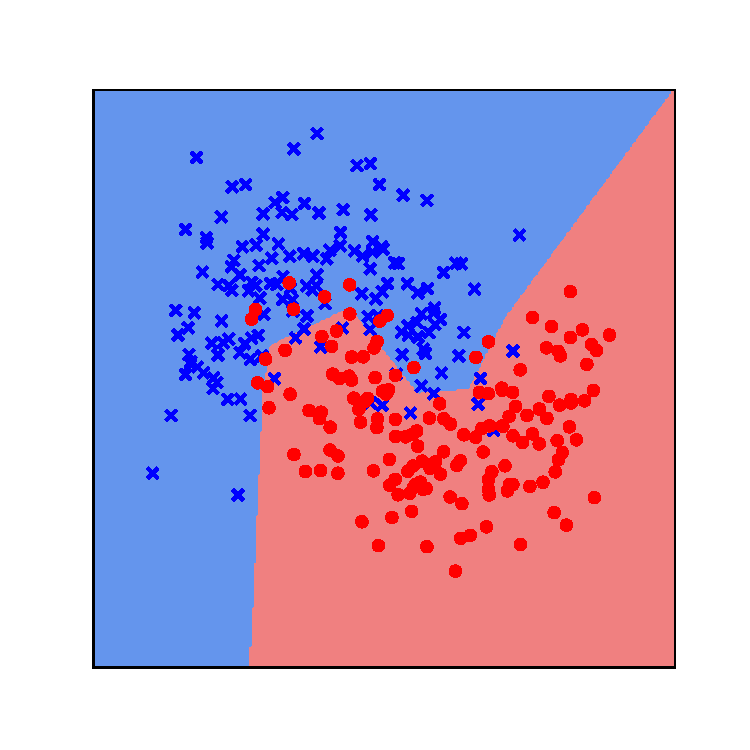
\includegraphics[width=0.98\textwidth]{figures/main/ch2-background/normal.pdf}
    \caption{Good fit}
    \label{figure:ch2-fitting_points_c}
  \end{subfigure}
  \caption{
    Decision boundary of three classifiers with different complexity for the same set of samples.
  }
  \label{figure:ch2-fitting_points}
\end{figure}


For a training sample $\Sset$, we denote $h_\Sset \in \mathrm{ERM}_{\Hset}(\Sset)$, one solution of applying $\mathrm{ERM}_\Hset$ on the set $\Sset$, if there exists multiple hypotheses with minimal error on the training sample, then the minimization problem returns an arbitrary one.
% In practice, the hypothesis class is chosen based on a hypothesis on the relation between the data and its label.
In practice, the hypothesis class is chosen on the basis of an assumption about the relationship between the data and its label.
For example, if the relation between the data and its label is supposedly linear then the hypothesis class can be the set of all linear functions.
This kind of restriction is called an \emph{inductive bias} because the learner is \emph{biased} toward a particular set of predictors.

The ERM paradigm assumes that a hypothesis $h_\Sset$ that minimizes the risk $R_\Sset$ will also minimize the true risk $R_\Dset$.
% This assumption mean that as the \emph{size} of the training set increases the minimization becomes more ``accurate'' or equivalently the empirical risk $R_\Sset(h)$ \emph{converge uniformly} to the actual risk $R_\Dset(h)$ over $h \in \Hset$.
% where the \emph{uniform convergence} is defined as follows:
% \begin{equation}
% 	\Pbb \left[ \sup_{h \in \Hset} \left| R_\Dset(h) - R_\Sset(h) \right| < \epsilon \right] \rightarrow 0 \quad \text{ when } \quad |\Sset| \rightarrow \infty, \quad \forall \epsilon > 0
% \end{equation}
To verify that this assumption is correct, we need to ensure that all hypotheses in the hypothesis class $\Hset$ are good approximators of their true risk.
We say that a hypothesis class has \emph{uniform convergence property} if there exists a function $m_\Hset:(0, 1)^2 \rightarrow \Nbb$ such that for every $\epsilon, \delta \in (0, 1)$, if $\Sset$ is a sample of $m \leq m_\Hset(\epsilon, \delta)$ examples drawn \emph{independent and identically} according to $\Dset$, then, with probability of at least $1 - \delta$:
\begin{equation} \label{equation:ch2-eps_representative}
  \forall h \in \Hset, \quad |R_\Dset(h) - R_\Sset(h)| \leq \epsilon \enspace,
\end{equation}
where the function $m_\Hset$, called \emph{the sample complexity}, measures the minimal number of examples needed to ensure that with probability of at least $1 - \delta$ the \Cref{equation:ch2-eps_representative} is verified.
The ``independent and identically distributed'' assumption is common in statistical learning theory.
It is easy to see that the error between $R_\Sset(h)$ and $R_\Dset(h)$ is dependent on how well $\Sset$ is representative of $\Dset$.
Therefore, the parameter $\delta$ characterizes the probability of having a nonrepresentative sample. We call $1 - \delta$ the \emph{confidence parameter} of our prediction.


% Therefore, we need to make the assumption that the training set $\Sset$ is a representative sample of the distribution $\Dset$.

The following result gives the sample complexity measure the maximum value for which the hypothesis class has \emph{uniform convergence property}.
\begin{theorem}[\citet{shalev2014understanding}] \label{theorem:ch2-sample_complexity_bound}
  Let $\Hset$ be a \emph{finite} hypothesis class, then $\Hset$ enjoys the uniform convergence property with sample complexity:
  \begin{equation}
      m_\Hset(\epsilon, \delta) \leq \left\lceil \frac{\log(2 |\Hset|	/ \delta)}{2 \epsilon^2} \right\rceil \enspace.
  \end{equation}
  \removespace
\end{theorem}
\noindent
Note that we can also write the bound from~\Cref{theorem:ch2-sample_complexity_bound} as follows, with probability $1 - \delta$, we have for all $h \in \Hset$:
\begin{equation}
  \underbrace{\vphantom{\sqrt{\frac{\log(|\Hset|/\delta)}{2 m_\Hset(\epsilon, \delta)}}} R_\Dset(h)}_{\text{Error}} \leq \underbrace{\vphantom{\sqrt{\frac{\log(|\Hset|/\delta)}{2 m_\Hset(\epsilon, \delta)}}} R_\Sset(h)}_{\text{Estimation Error}} + \underbrace{\sqrt{\frac{\log(|\Hset|/\delta)}{2 m_\Hset(\epsilon, \delta)}}}_{\text{Complexity penality}} \enspace.
\end{equation}
This bound is called a \emph{generalization bound} and consists in bounding the true error by the empirical error and a complexity penalty.
In the above theorem, the condition on the finiteness of the hypothesis class might by too strong.
For example, if we consider the set of linear functions parameterized by a set of real-valued parameters the hypothesis class is infinite and the theorem above does not apply.
To characterize the learnability of infinite hypothesis classes, several complexity measures have been proposed.
One of the first, discovered by~\citet{vapnik2015uniform}, relies on a combinatorial notion called the Vapnik-Chervonenkis dimension (VC-dimension). They showed that having a finite VC-dimension is a necessary and sufficient condition for the uniform convergence property.
In the same vein, the Rademacher complexity~\cite{koltchinskii2000rademacher}, measures the richness of a class of real-valued functions with respect to a probability distribution.
In \Cref{subsection:ch2-recent_results_on_the_theory_of_neural_networks}, we will study recent generalization bounds specific to neural networks where the complexity penalty is dependent on the Lipschitz constant of the weights matrices.


A fundamental question of the ERM paradigm remains: \emph{how to choose the correct hypothesis class for which $\text{ERM}_\Hset$ will not lead to overfitting?} 
We answer this question by decomposing the true risk into two different components as follows: 
\begin{equation} \label{equation:ch2-bias_complexity_tradeoff}
  R_\Dset (h_\Sset) = 
  \underbrace{\left[ \min_{h \in \Hset} R_\Dset(h) \right]}_{\text{\scriptsize Approximation Error}} + \quad 
  \underbrace{\left[ R_\Dset(h_\Sset) - \min_{h \in \Hset} R_\Dset(h) \right]}_{\text{\scriptsize Estimation Error}} 
\end{equation}
\begin{itemize}
  \item \textbf{Approximation Error}: The approximation error corresponds to the minimum risk achievable by a classifier in the given hypothesis class.
  Intuitively, this error measures the quality of the hypothesis class and therefore the quality of the prior knowledge.
  Enlarging the hypothesis class, \ie, allowing more complex functions, can decrease the approximation error.
  \item \textbf{Estimation Error}: The estimation error is the difference between the approximation error and the error made by the ERM predictor.
  Recall that the empirical risk is only an estimate of the true risk.
  This error is dependent on the sample size and the complexity of the hypothesis class.
\end{itemize}
Recall that the main goal is to minimize the true risk $R_\Dset (h_\Sset)$, however, \Cref{equation:ch2-bias_complexity_tradeoff} shows a trade-off called the \emph{bias-complexity trade-off}.
The trade-off is as follows: if we choose a large and complex hypothesis space, we reduce the approximation error but at the same time we can increase the estimation error because a complex hypothesis space might lead to overfitting.
Conversely, choosing a small hypothesis space might reduce the estimation error but increase the approximation error leading to an \emph{underfitting} phenomenon.
We can illustrate the \emph{overfitting} and \emph{underfitting} phenomenons with \Cref{figure:ch2-fitting_points} which shows the decision boundary of 3 classifiers for the same set of samples.
\Cref{figure:ch2-fitting_points_a} shows a classifier which \emph{underfit} the data, meaning the decision boundary is not complex enough to separate the data correctly.
\Cref{figure:ch2-fitting_points_b} shows a classifier that almost perfectly follows the training data but is likely to have a higher error rate on the unseen data.
Finally, \Cref{figure:ch2-fitting_points_c} shows a classifier that seems to have a good compromise between the two.


As seen above, defining a small hypothesis class might lead to underfitting and a large hypothesis class might lead to overfitting.
A good way to balance the trade-off would be to minimize the empirical risk while also minimizing the complexity of the hypothesis class.
Let us define a \emph{regularization} function $r: \Hset \rightarrow \Rbb$ which takes a hypothesis as input and a measure of the ``complexity'' of the hypothesis.
We could now update the learning rule as follows:
\begin{equation}
  \argmin_{h \in \Hset} \left[ R_\Sset(h) + r(h) \right]
\end{equation}
This learning rule minimizes the empirical risk $R_\Sset(h)$ and the regularization function $r$. If $r(\ \cdot\ )$ is carefully chosen, this prevent overfitting and improve generalization on unseen data.
This learning rule is closely related to \emph{Structural Minimization Paradigm} (SRM) \cite{shalev2014understanding}.
In the next section, we will present a classical regularization function for neural networks and we will introduce a new regularization scheme in \Cref{chapter:ch5-lipschitz_bound}.




% A good way to offset a large hypothesis class would be to specific preference over hypothesis within the hypothesis class.
% The \emph{Structural Minimization Paradigm} (SRM) assumes that the hypothesis class can be written as the union of multitude smaller hypothesis class as follows: $\Hset = \bigcup_{n \in \Nbb} \Hset_n$ with a weight function $w: \Nbb \rightarrow [0, 1]$ which assigns a weight to each hypothesis class, $\Hset_n$, such that a higher weights reflects a lower preference for the hypothesis class.
% Intuitively, the weight function is a measure of the ``complexity'' of the hypotesis.
% The SRM learning paradigm can then be defined as follows:
% \begin{equation}
%   \text{SRM}_\Hset \in \argmin_{h \in \Hset, n \in \Nbb} \left[ R_\Sset(h) + w(n) \right]
% \end{equation}
% The SRM learning paradigm minimizes the empirical risk $R_\Sset(h)$ and the weight function $w$; therefore, ovoiding overfitting and improving generalization by reducing the complexity of the hypotesis while maintening a low empirical risk.
% In the next section, we will present neural networks which are the type of function we will use as predictors and we will see how to implement the ERM and SRM paradigm.









% \‰\‰\‰
%
% The ERM paradigm with inductive bias is based on an important assumption.
% We assume that uniformly over all $h \in \Hset$, the empirical risk is close to the true risk, meaning, an $h$ that minimize the empirical risk with respect to a data set $\Sset$ will also minimize the \emph{true} risk.
% More formally, 
% \begin{equation}
%   \forall h \in \Hset, \quad \left| R_\Sset(h) - R_\Dset(h) \right| \leq \epsilon \enspace.
%   \label{equation:ch2-eps_respresentative_sample} 
% \end{equation}
% If this assumption is met, then the ERM paradigm will always return a good classifier.
% \begin{lemma}[Lemma 4.2 \citet{shalev2014understanding}] 
%   If \Cref{equation:ch2-eps_respresentative_sample} hold, then any output of $\mathrm{ERM}_\Hset(\Sset)$, namely, any $h_\Sset \in \argmin_{h \in \Hset} R_\Sset(h)$, satisfies
%   \begin{equation}
%     R_\Dset(h_\Sset) \leq \min_{h \in \Hset} R_\Sset(h) + 2\epsilon
%   \end{equation}
% \end{lemma}
%
% \‰\‰\‰


% Let us consider an input space $\Xset = [0, 1]^d$ of dimension $d$, an output space $\Yset = [k]$ where $k$ is the number of class and a data distribution $\Dset$ over $\Xset \times \Yset$.
% We seek to find a function $h: \Xset \rightarrow \Yset$ that maps the input $\xvec \in \Xset$ to the output $y \in \Yset$ with $h \in \Hset$ where $h$ is called the \emph{hypothesis} and $\Hset$ the \emph{hypothesis space}.
% in order to measure how well the function fits, we de\emph{loss function} $l: \mathcal{y} \times \mathcal{y} \rightarrow \rbb^{+}$ is defined.
% The \emph{risk} $R$ associated with the hypothesis $h(\xvec)$ is defined as follows:
% \begin{equation}
%   R(h) \triangleq \Ebb_{(\xvec, y) \sim \Dset}\  L \left( h(\xvec), y \right)
% \end{equation}
% The goal of a \emph{learning algorithm} is to find a hypothesis $h^* \in \Hset$ which minimize the risk $R(h)$:
% \begin{equation}
%   h^* \triangleq \argmin_{h \in \Hset} R(h) .
% \end{equation}

% In practice, the joint probability distribution $\Dset$ is unknown.
% Instead, we have $n$ independent observations of the distribution called the \emph{training set}
% \begin{equation}
%   \mathcal{T} \triangleq \left\{ \left(\xvec^{(1)}, y^{(1)} \right), \dots, \left( \xvec^{(n)}, y^{(n)} \right) \right\} ,
% \end{equation}
% where $\xvec \in \Xset$ and $y \in \Yset$.

% The risk minimization problem is therefore replace by the \emph{empirical risk minimization} as follows:
% \begin{equation}
%   E(h, n) \triangleq \frac{1}{n} \sum_{i = 1}^{n} L\left(h\left(\xvec^{(i)}\right), y^{(i)}\right) ,
% \end{equation}
% the learning algorithm then becomes:
% \begin{equation}
%   \hat{h}^* \triangleq \argmin_{h \in \Hset} E(h, n)  .
% \end{equation}


% \paragraph{Structural Risk Minimization} (SRM).
% The ERM principle assumes that the function $\hat{h}^*$ minimizing $E(h, n)$ leads to the risk $R(\hat{h}^*)$ being close to the minimum.
% This assumption mean that as the \emph{size} of the training set increase the minimization becomes more accurate.
% More formally, the ERM principle assumes that $R(\hat{h}^*)$ converge to its minimum value on the set $h \in \Hset$ when $n \rightarrow \infty$.
% \citet{Vapnik1991TheNA} have shown that this equivalent to say that the empirical risk $E(h, n)$ \emph{converge uniformly} to the actual risk $R(h)$ over $h \in \Hset$ where the \emph{uniform convergence} is defined as follows:
% \begin{equation}
%   \Pbb \left[ \sup_{h \in \Hset} \left| R(h) - E(h, n) \right| < \epsilon \right] \rightarrow 0 \quad \text{ when } \quad n \rightarrow \infty, \quad \forall \epsilon > 0 
% \end{equation}


% \citet{Vapnik1991TheNA} have shown that this assumption is equivalent to the following: does the empirical risk $E(h, n)$ \emph{converge uniformly} to the actual risk $R(h)$ over $h \in \Hset$ where the \emph{uniform convergence} is defined as follows:
% \begin{equation}
%   \Pbb \left[ \sup_{h \in \Hset} \left| R(h) - E(h, n) \right| < \epsilon \right] \rightarrow 0 \quad \text{ when } \quad n \rightarrow \infty, \quad \forall \epsilon > 0 
% \end{equation}


% However, does increasing the \emph{size} of the training set allow a better minimisation of the actual risk.
% More formally, does $R(\hat{h}^*)$ converge to its minimum value on the set $h \in \Hset$ when $n \rightarrow \infty$.

% \citet{vapnik1992principles} 

% The 0-1 loss function is a natural loss function to use because it assigns 0 for a correct classification and 1 for an incorrect classification.


% of the ERM principle \ie, does $R(\hat{h}^*)$ converge to its minimum value on the set $h \in \Hset$ when $n \rightarrow \infty$ is equivalent to the question: 

% is equivalent to the question: does the empirical risk E(h, n) \emph{converge uniformly} to the actual risk $R(h)$ over $h \in \mat

% \begin{equation}
%   h^* = \argmin_{h \in \Hset} \frac{1}{n} \sum_{i = 0}^{n} L(h(\xvec_i), y) + \lambda C(\theta) 
% \end{equation}

% Because the relation between $\xvec \in \Xset$ and $y \in \Yset$ is unknown, we aim to find the best approximation of the function $h$ with a parameterized function $h_\theta \in \Hset$ where $\Hset$ is called the \emph{hypothesis space}.

% The goal of a \textbf{learning algorithm} is to learn a function $f: \Xset \rightarrow \Yset$ which outputs $y \in \Yset$ given an input $\xvec \in \Xset$ with $f \in \Hset$ where $\Hset$ is called the \emph{hypothesis space}.

% The supervised learning settings assume that a function $f: \Xset \rightarrow \Yset$ exists.

% The supervised learning settings assume that a function $f$ that maps $\xvec \sim \Xset$ to $y \sim \mathcal{y}$ exists.

% The goal of a \textbf{learning algorithm} is to approximate $f$ by a parameterized function $f_\theta$.
% The standard method to learn the set of parameters $\theta$ is the \textbf{empirical risk minimization (ERM)}:
% \begin{equation*}
%   \hat{\theta}_{ERM} \triangleq \argmin_{\theta} \frac{1}{n} \sum_{i=1}^{n} L (f_{\theta} (\xvec_i), y_i )
% \end{equation*}

% \begin{equation}
%   \min_{\theta} \Ebb_{(\xvec, y) \sim \Dset} \left[ L(f_\theta(x), y) \right].
% \end{equation}

%%%%%%%%%%%%%%%%%%%%%%%%%%%%%%%%%%%%%%%%%%%%%%%%%%%%%%%%%%%%%%%%%%%%%%%%%%%%%%%
\subsection{Preliminaries on Neural Networks}
\label{subsection:ch2-preliminaries_on_neural_networks}
%%%%%%%%%%%%%%%%%%%%%%%%%%%%%%%%%%%%%%%%%%%%%%%%%%%%%%%%%%%%%%%%%%%%%%%%%%%%%%%


% \begin{figure}[ht]
%   \centering
%   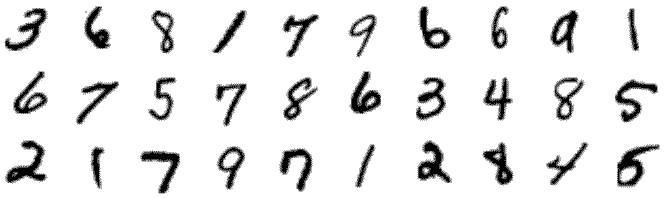
\includegraphics[width=0.88\textwidth]{figures/main/ch2-background/mnist-dataset.png}
%   \caption{Images with handwritten digits in the MNIST database \cite{lecun1998gradient}}
%   \label{figure:ch2-mnist-database}
% \end{figure}
%
% In \citeyear{lecun1998gradient}, \citeauthor{lecun1998gradient} had successfully learned a function capable of recognizing handwritten digits in images.
% They used the MNIST dataset \cite{lecun1998gradient} consisting of black and white images of size $28 \times 28$ pixels (\Cref{figure:ch2-mnist-database} presents a sample of images from the MNIST database).
% Their goal was to develop an algorithm that takes a vector as input and produces one digit from 0 to 9 as the output.
% Although simple for a human, this task is a non-trivial problem for computers due to the uniqueness of each image.
% To solve this problem, \citet{lecun1998gradient} trained a neural network based on the images of the MNIST dataset and their labels.

% This is a non-trivial problem because each image is unique and while digits can be differentiated based on their shapes and strokes, these features give poor results for an automated system.

% In the previous section, we said that we restrict the learner towards a specific set of predictors.
% In this thesis, we focus on neural networks.
Neural networks, which find their roots in the work of \citet{mcculloch1943logical,rosenblatt1958perceptron}, can be analytically described as a composition of linear functions interlaced with nonlinear functions (also called activation functions).
A feedforward neural network can be defined as follows:

% \begin{definition}[Neural Network]
%   Given a depth $\depth \in \Nbb$, 
%   let $w = \{ w^{(i)} \}_{i \in [\depth]}$ and $b = \{ b^{(i)} \}_{i \in [\depth]}$ be sequences of ``dimension'',  
%   $\weights = \left\{ \left( \Wmat^{(i)}, \bvec^{(i)} \right) \right\}_{i \in [\depth]}$ a set of weights matrices and bias vectors 
%   such that $\Wmat^{(i)} \in \Rbb^{w^{(i)}}$ and $\bvec^{(i)} \in \Rbb^{b^{(i)}}$ and 
%   sequence of activation functions $\act = \{\act_i \}_{i \in [\depth]}$.
% %   Let $\dim^{w} = \{ \dim_1^w, \dots, \dim_\depth^w \}$ and $\dim^{b} = \{ \dim_1^b, \dots, \dim_\depth^b \}$ 
% % be sequences of ``dimension'', let $\dim_{\text{in}} = \dim_\depth^w$ and $\dim_{\text{out}} = \dim_\depth^w$.
%   Let $\Xset \subset \Rbb^{\dim_{\text{in}}}$ and 
%   $\Yset \subset \Rbb^{\dim_\text{out}^w}$ be the input space and output space respectively.
%   % Given a depth $\depth$, a set of weights matrices and bias vectors $\weights = \left\{ \left( \Wmat^{(i)}, \bvec^{(i)} \right) \right\}_{i \in [\depth]}$ and a sequence of activation functions $\act = \{\act_i \}_{i \in [\depth]}$, a neural network is a function $N^\act_\weights : \Xset \rightarrow \Yset$ such that
%   A neural network is a function $N^\act_\weights : \Xset \rightarrow \Yset$ such that
%   \begin{equation}
%     \nn^\act_{\weights}(\xvec) \triangleq \layer^{\act_\depth}_{\Wmat^{(\depth)}, \bvec^{(\depth)}} \circ \cdots \circ \layer^{\act_1}_{\Wmat^{(1)}, \bvec^{(1)}}(\xvec)
%   \end{equation}
%   % where $d$ corresponds to the depth of the network (\ie, the number of layers), $\weights$ is the set of weights matrices and bias vectors $\weights = \left\{ \left( \Wmat^{(1)}, \bvec^{(1)} \right) \dots \left( \Wmat^{(d)}, \bvec^{(d)} \right) \right\}$.
%   % $\Bmat$ is the set of bias vectors $\Bmat = \left\{ \right\}$.
%   where $\layer^{\act_i}_{\Wmat^{(i)},\bvec^{(i)}}: \Rbb^{w^{(i)}} \rightarrow \Rbb^{w^{(i+1)}}$ (also called layer) is a function parameterized by the weight matrix $\Wmat^{(i)}$, the bias vector $\bvec^{(i)}$ and the activation function $\act_i$ and can be expressed as follows: 
%   \begin{equation}
%     \layer^{\act_i}_{\Wmat^{(i)},\bvec^{(i)}} (\xvec) \triangleq \act_i \left(\Wmat^{(i)}\xvec + \bvec^{(i)}\right)
%   \end{equation}
% \end{definition}

\begin{definition}[Neural Network] \label{definition:ch2-neural_networks}
  Given a depth $\depth \in \Nbb$, 
  let $\dimw = \{ \dimw^{(i)} \}_{i \in [\depth+1]}$ and $\dimb = \{ \dimb^{(i)} \}_{i \in [\depth]}$ be sequences of integers, $\weights = \left\{ \left( \Wmat^{(i)}, \bvec^{(i)} \right) \right\}_{i \in [\depth]}$ a set of weights matrices and bias vectors 
  such that $\Wmat^{(i)} \in \Rbb^{\dimw^{(i)} \times \dimw^{(i+1)}}$ and $\bvec^{(i)} \in \Rbb^{\dimb^{(i)}}$ and a sequence of activation functions $\act = \{\act_i \}_{i \in [\depth]}$.
  Let $\Xset \subset \Rbb^{\dimw^{(1)}}$ and $\Yset \subset \Rbb^{\dimw^{(\depth+1)}}$ be the input and output spaces respectively.
	$\dimw^{(1)}$ and $\dimw^{(\depth)}$ refer to the input and output dimension respectively.
  % $\dimw^{(1)}$ refers to the input dimension and $\dimw^{(\depth)}$ refers to the output dimension.
  A neural network is a function $\nn^\act_\weights : \Xset \rightarrow \Yset$ such that
  \begin{equation}
    \nn^\act_{\weights}(\xvec) \triangleq \layer^{\act_\depth}_{\Wmat^{(\depth)}, \bvec^{(\depth)}} \circ \cdots \circ \layer^{\act_1}_{\Wmat^{(1)}, \bvec^{(1)}}(\xvec)
  \end{equation}
  where $\layer^{\act_i}_{\Wmat^{(i)},\bvec^{(i)}}: \Rbb^{w^{(i)}} \rightarrow \Rbb^{w^{(i+1)}}$ (also called layer) is a function parameterized by the weight matrix $\Wmat^{(i)}$, the bias vector $\bvec^{(i)}$ and the activation function $\act_i$.
  $\layer^{\act_i}_{\Wmat^{(i)},\bvec^{(i)}}:$  is defined as follows: 
  \begin{equation}
    \layer^{\act_i}_{\Wmat^{(i)},\bvec^{(i)}} (\xvec) \triangleq \act_i \left(\Wmat^{(i)}\xvec + \bvec^{(i)}\right) \enspace,
  \end{equation}
  and $\rho_\depth$ is identity function.
\end{definition}

\noindent
Based on this definition, for a given training set $\Sset \subset \Xset \times \Yset$, a set of activation functions $\act$, a set of weights and biases $\weights$ and a loss function $L: \Yset \times [k] \rightarrow \Rbb_+$, the ERM learning paradigm for neural networks is given by
\begin{equation} \label{equation:ch2-erm_neural_network}
  \argmin_{\weights} \frac{1}{|\Sset|} \sum_{(\xvec, y) \in \Sset} L(N^\act_\weights(\xvec), y) 
\end{equation}
For classification problems, the zero-one loss is non-convex, and finding a near optimal solution is an NP-hard problem~\cite{feldman2012agnostic,bendavid2003difficulty}.
Instead, a common approach is to use a surrogate such as the logistic loss multiclass function and estimate the parameters by maximizing the \emph{likelihood} over the data.
This loss $L:\Yset \times [k]$, is defined as follows:
\begin{equation}
  L(N^\rho_\Omega(\xvec), y) = -\log
    \left(
      \frac
        {e^{\left(N^\rho_\Omega(\xvec)\right)_y}}
	{\sum_{j\in[k]} e^{\left(N^\rho_\Omega(\xvec)\right)_j}}
    \right)
\end{equation}
The generic approach for minimizing the empirical risk in \Cref{equation:ch2-erm_neural_network} is by \emph{gradient descent} with the \emph{backpropagation} algorithm ~\cite{rumelhart1986learning} which consists in computing the gradient with the chain-rule.




% Instead, a common approach is to used the softmax activation function as the last nonlinear activation $\act_d$ with the cross-entropy loss function and estimate the parameters with \emph{maximum likelihood}~\cite{hastie2009elements}.
% The softmax activation function, $\act_d: \Rbb^k \rightarrow [0, 1]^k$, is defined as follows:
% \begin{equation}
%   \leftmat \act_d(\xvec) \rightmat_i = \frac{e^{\xvec_i}}{\sum_{j=0}^{k-1} e^{\xvec_j}}, \quad \forall i
% \end{equation}
% The generic approach for minimizing the empirical risk in \Cref{equation:ch2-erm_neural_network} is by \emph{gradient descent} with the \emph{backpropgation} algorithm ~\cite{rumelhart1986learning} which consists of computing the gradient with the help of the chain-rule.


As seen in the previous section, the SRM paradigm minimizes two terms, the empirical risk and a weight function measuring the ``complexity'' of the hypothesis.
% It has been shown that the number of free parameters can be used as a measure of complexity and a number of work have proposed techniques to reduce the number parameters~\cite{lecun1990optimal,thodberg1991improving,weigend1991generalization}.
% However, a different way of constraining the complexity is to limit the growth of weights~\cite{hinton1987learning}.
% This \emph{regularization} \cite{tikhonov1977solutions,krogh1992simple}, also called \emph{weight decay}, prevents weights from growing too large unless it is necessary.
It has been shown that the $\ell_2$ norm of the weights of a network can be used as an adequate measure of complexity \cite{hinton1987learning}.
% However, a different way of constraining the complexity is to limit the growth of weights~\cite{hinton1987learning}.
This \emph{regularization} \cite{tikhonov1977solutions}, also called prevents weights from growing too large unless.
The SRM learning algorithm can then be expressed as follows:
\begin{equation}
  \argmin_{\weights} \frac{1}{|\Sset|} \sum_{(\xvec, y) \in \Sset} L(N^\act_\weights(\xvec), y) + \lambda \sum_{(\Wmat, \bvec) \in \weights} \left( \norm{\Wmat}_\mathrm{F} + \norm{\bvec}_\mathrm{2} \right)
\end{equation}
where $\lambda > 0$ is the regularization parameter.


\begin{figure}[ht]
  \centering
  \begin{subfigure}[b]{0.32\textwidth}
    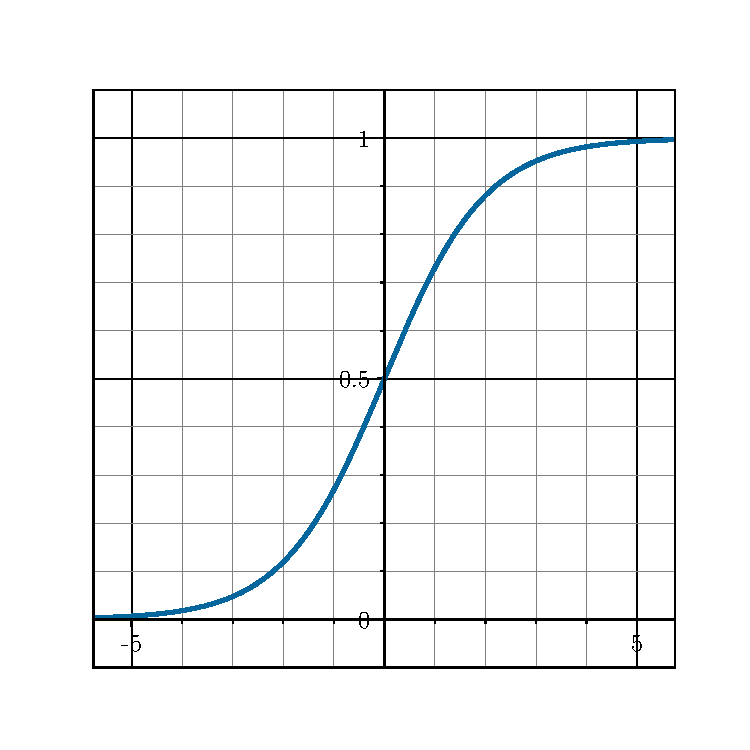
\includegraphics[width=0.98\textwidth]{figures/main/ch2-background/sigmoid.pdf}
    \caption{Sigmoid Activation}
  \end{subfigure}
  \hfill
  \begin{subfigure}[b]{0.32\textwidth}
    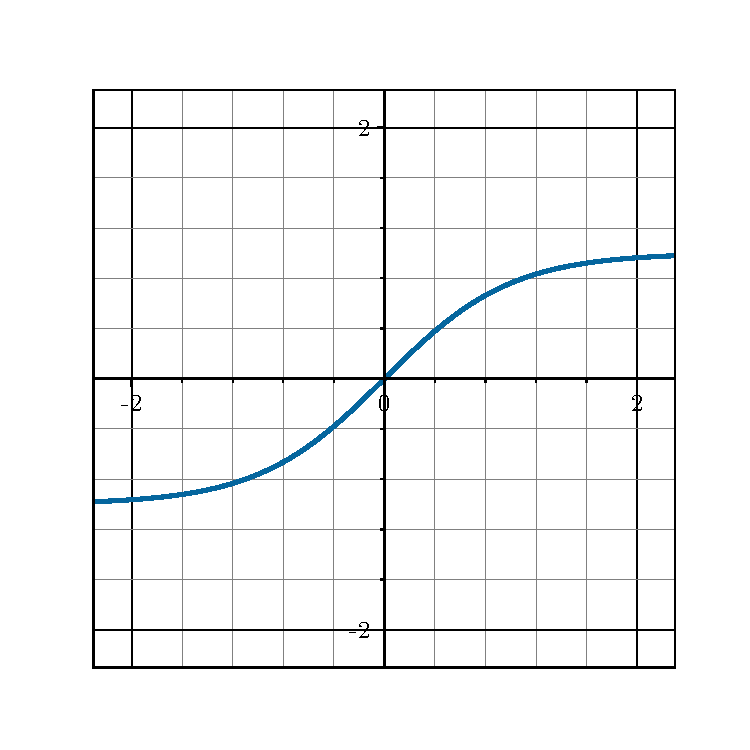
\includegraphics[width=0.98\textwidth]{figures/main/ch2-background/tanh.pdf}
    \caption{Tanh Activation}
  \end{subfigure}
  \hfill
  \begin{subfigure}[b]{0.32\textwidth}
    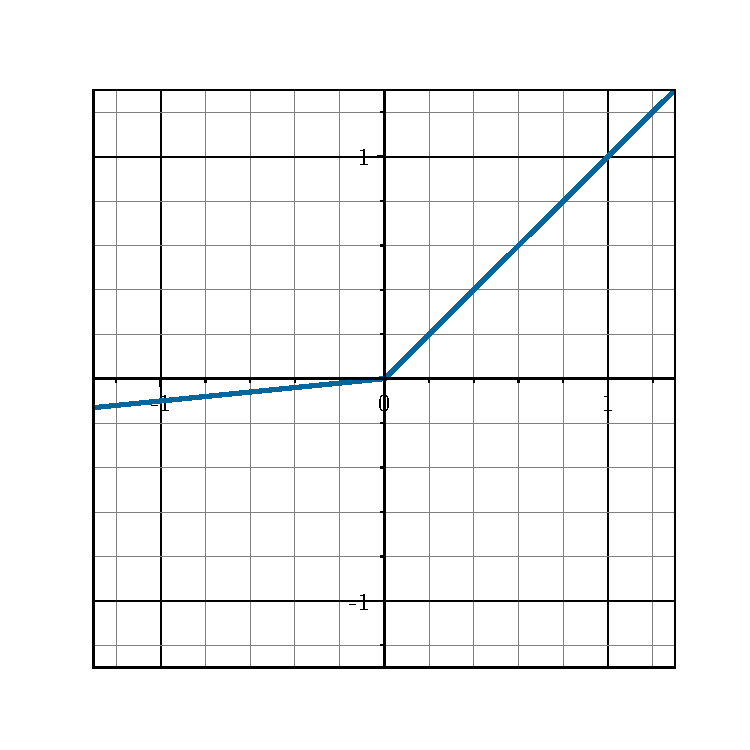
\includegraphics[width=0.98\textwidth]{figures/main/ch2-background/relu.pdf}
    \caption{Leaky-ReLU Activation}
  \end{subfigure}
  \caption{Graphical representation of three common activation functions}
  \label{figure:ch2-activation_functions}
\end{figure}


Choosing the right activation function has been an active area of research.
Hereafter, we present three common activation functions used by practitioners.
\begin{itemize}
  \item \textbf{Sigmoid activation} \cite{han1995influence}
    \begin{equation*}
      \act(x) = \frac{1}{1+e^{-x}} 
    \end{equation*}
    The sigmoid activation function is one of the first continuous nonlinear functions to be used in the context of neural networks.
		It takes a real value as input and outputs another value between 0 and 1.
  \item \textbf{Hyperbolic Tangent activation} \cite{karlik2011performance}
    \begin{equation*}
      \act(x) = \frac{e^x - e^{-x}}{e^x + e^{-x}}
    \end{equation*}
    The hyperbolic tangent activation function is similar to the sigmoid activation function but instead of returning between 0 and 1, the function returns values between -1 and 1.
  \item \textbf{Rectified Linear activation (ReLU)} \cite{nair2010rectified,maas2013rectifier}
    \begin{equation*}
      \act(x) = \max(0, x)
    \end{equation*}
    The ReLU activation was proposed to avoid the \emph{vanishing gradient problem}.
    The vanishing gradient problem, discovered by \citet{bengio1994learning}, occurs with hyperbolic tangent or sigmoid activation when the magnitude of the values is almost saturated at $-1$ or $1$, in this case the gradient is close to $0$ and difficulties of optimization and convergence occur.
    The ReLU activation addresses this problem due to the simple values of its gradients which are either 0 or 1 on $\Rbb_-$ or $\Rbb_+$ respectively.
    Furthermore, it has the advantage to be less computationally expensive than tanh and sigmoid because it involves simpler mathematical operations.
  \item \textbf{Leaky Rectified Linear activation (Leaky-ReLU)} \cite{maas2013rectifier}
    \begin{equation*}
      \act(x) = \max(\alpha, x)
    \end{equation*}
    More recently, the Leaky-ReLU ($\alpha > 0$) activation function was proposed.
    It introduces the parameter $\alpha$ which characterizes the slope on $\Rbb_-$.
    The use of Leaky-ReLU with a small constant $\alpha$ tends to facilitate convergence of very deep architectures.
\end{itemize}

\noindent
\Cref{figure:ch2-activation_functions} presents the graphical representation of the activation functions presented above.
In this thesis, we will use the Leaky-ReLU function with different $\alpha$ when we train deep neural networks.
We simplify the notation $\nn^\act_\weights$ with $\nn_\weights$.




% From $\mathcal{N}$, we can easily build a deep ReLU network $\mathcal{N'}$ of width exactly $n+3$, such that $\forall x \in [0,1]^{n+3}$, $\left|f(\xvec_{1} \ldots \xvec_{n}) - \left(\mathcal{N}'\left(\xvec\right)\right)_{1}\right| < \epsilon$.
% Thanks to \Cref{lemma:dcnn_approx_neural_network}, this last network can be approximated arbitrarily well by a DCNN of width $n+3$.
%
% \begin{theorem}
%   Let $\Xset \subset \Rbb^{w_{(1)}}$.
%   For any continuous function $f: \Xset \rightarrow \Rbb^{w^{(\depth)}}$, then there exists a  
%
%   Let $\Xset \subset \Rbb^{w_{(1)}}$ and let $f: \Rbb^{w^{(1)}} \rightarrow \Rbb^{w^{(\depth)}}$ be a continuous function.
%   Then, there exists a neural networks parameterized by $\weights$ with an input dimension $w^{(1)}$, an arbitrary depth $\depth$, and $\relu$ activation such that:
%   \begin{equation}
%     \norm{f(\xvec) - \nn(\xvec)} \leq \epsilon
%   \end{equation}
%   \label{theorem:ch2-universal_approximation_theorem}
% \end{theorem}
%


% \citet{cybenko1989approximation} have shown that shallow neural networks with sigmoid activation can \emph{theoretically} approximate any decision boundary.
%
% The arbitrary depth case was also studied by number of authors, such as Zhou Lu et al in 2017,[11] 
% \cite{lu2017expressive}
%
% Boris Hanin and Mark Sellke in 2018,[12] 
% \cite{hanin2017universal}



%%%%%%%%%%%%%%%%%%%%%%%%%%%%%%%%%%%%%%%%%%%%%%%%%%%%%%%%%%%%%%%%%%%%%%%%%%%%%%%
\subsection{Adversarial Attacks \& Robustness of Neural Networks}
\label{subsection:ch2-adversarial_attacks_robustness_of_neural_networks}
%%%%%%%%%%%%%%%%%%%%%%%%%%%%%%%%%%%%%%%%%%%%%%%%%%%%%%%%%%%%%%%%%%%%%%%%%%%%%%%


As seen in the introduction (\Cref{chapter:ch1-introduction}), deep neural networks achieve state-of-the-art performances in a variety of domains such as natural language processing~\cite{radford2018Language}, image recognition~\cite{he2016deep} and speech recognition~\cite{hinton2012deep}.
However, it has been shown that such neural networks are vulnerable to \emph{adversarial examples}, \ie, imperceptible variations of the natural examples, crafted to deliberately mislead the models~\cite{globerson2006nightmare,biggio2013evasion,szegedy2013intriguing}.
Because it is difficult to characterize the space of visually imperceptible variations of a natural image, existing adversarial attacks use $\ell_p$ norms as surrogate measures.
We can formally define an adversarial example as follows:
\begin{definition}[Adversarial Pertubation]
  Given an example $\xvec$ and its label $y$, a trained neural network $\nn_\weights$ with $\argmax_i \{ \nn_\weights(\xvec)_i \} = y$ and a radius $\epsilon \in \Rbb$, an adversarial perturbation is a vector $\adv \in \Xset$ such that:
  % Given a dataset $\Sset \subset \Xset \times \Yset$, a pair $(\xvec, y) \in \Sset$ and a trained neural network $\nn_\weights$ on $\Sset$ such that $\argmax_{i} \{ \nn_\weights(\xvec)_i \} = y$, let $\adv \in \Xset$ be an adversarial perturbation such that:
  \begin{align}
    &\argmax_{i} \{ \nn_\weights (\xvec + \adv)_i \} \neq y \\
    &\st\ \norm{\adv}_p \leq \epsilon \notag
  \end{align}
  where $\epsilon$ is a small value defined by the attacker.
\end{definition}

Note that this definition assumes that the attacker (the person crafting the attack) has access to the parameters of the model.
Typically, an attack method is either \emph{white-box} (complete knowledge of the model and its parameters) or \emph{black-box} (no knowledge of the model).
It is possible to consider that the white-box setting admits too strong assumptions because a model and its parameters could very well be hidden from the public.
In general, it is safer to assume that the adversary has complete knowledge of the model and its defense.
This principle is known in the field of security as Kerckhoffs’ principle~\cite{kerckhoffs1883cryptographie} or Shannon's maxim~\cite{shannon1949communication}.
Therefore, in this thesis, we only consider defenses against white-box attacks which imply robustness against black-box adversaries.


%%%%%%%%%%%%%%%%%%%%%%%%%%%%%%%%%%%%%%%%%%%%%%%%%%%%%%%%%%%%%%%%%%%%%%%%%%%%%%%
\subsubsection{Implementing Adversarial Attacks}
\label{subsubsection:ch2-adversarial_attacks}
%%%%%%%%%%%%%%%%%%%%%%%%%%%%%%%%%%%%%%%%%%%%%%%%%%%%%%%%%%%%%%%%%%%%%%%%%%%%%%%

Since the discovery of adversarial perturbations, a variety of procedures, \aka \emph{adversarial attacks}, have been developed to generate adversarial examples.
% for example FGSM \cite{goodfellow2014explaining}, PGD \cite{madry2018towards} and C\&W \cite{carlini2017towards}, to mention the most popular ones.
FGSM \cite{goodfellow2014explaining}, PGD \cite{madry2018towards} and \cite{carlini2017towards} to name a few, are the most popular ones.
To find the best perturbation $\adv$, existing attacks can adopt one of the two following strategies:
% \begin{itemize}
%   \item \textbf{Loss maximization}: maximizing the loss $L(\nn_\weights(\xvec + \adv), y)$ under some constraint on $\norm{\adv}_p$ with $p \in \{0, \dots, \infty\}$.;
%   \item \textbf{Perturbation minimization}: minimizing $\norm{\adv}_p$ under some constraint on the loss $L(\nn_\weights(\xvec + \adv), y)$.
% \end{itemize}

\paragraph{Loss maximization.}
In this scenario, the procedure maximizes the loss objective function $L(\nn_\weights(\xvec + \adv), y)$, under the constraint that the $\lp$ norm of the perturbation remains bounded by some value $\epsilon$, as follows:
\begin{equation} \label{equation:ch2-lossmax}
  \argmax_{\adv:\norm{\adv}_p \leq \epsilon} L(\nn_\weights(\xvec + \adv), y) \enspace.
\end{equation}
The typical value of $\epsilon$ depends on the norm $\norm{\ \cdot\ }_p$ considered in the problem setting.
% In order to compare $\linf$ and $\ltwo$ attacks of similar strength, we choose values of $\epsilon_\infty$ and $\epsilon_2$ (for $\linf$ and $\ltwo$ norms respectively) which result in $\linf$ and $\ltwo$ balls of equivalent volumes.
% For the particular case of CIFAR-10, this would lead us to choose $\epsilon_\infty = 0.03$ and $\epsilon_2 = 0.8$ which correspond to the maximum values chosen empirically to avoid the generation of visually detectable perturbations.
The current state-of-the-art method to solve \Cref{equation:ch2-lossmax} is based on a projected gradient descent (PGD)~\cite{madry2018towards} of radius~$\epsilon$.
Given a budget $\epsilon$, it recursively computes
\begin{equation} \label{equation:ch2-projectionPGD}
  \xvec^{(t+1)} = \prod_{\mathcal{B}_p(\xvec,\epsilon)}\left(\xvec^{(t)}
    + \alpha \argmax_{\adv: \norm{\adv}_p \leq 1} \adv^\top \nabla_{\xvec^{(t)}} L\left( \nn_\weights \big(\xvec^{(t)} \big), y \right)
\right)
\end{equation}
where $\Bset_p(\xvec,\epsilon) = \{ \xvec + \adv:\norm{\adv}_p \leq \epsilon\}$ is the ball of norm $p$ with radius $\epsilon$, centered at $\xvec$, $\alpha$ is a gradient step size, and $\prod_\Bset$ is the projection operator on the ball $\Bset$.
The PGD attack is currently used in the literature with $p=2$ and $p=\infty$.
The attack with the norm $p=\infty$ is state-of-the-art for the loss maximization problem.

\paragraph{Perturbation minimization.}
This type of procedure searches for the perturbation with the minimal $\lp$ norm, under the constraint that $L(\nn_\weights(\xvec + \adv), y)$ is bigger than a given bound $c$:
\begin{align}
  &\argmin_{\adv} \norm{\adv}_p \label{equation:ch2-normmin} \\
  &\st\ L(\nn_\weights(\xvec + \adv), y) \geq c \notag
\end{align}
The value of $c$ is typically chosen depending on the loss function $L$.
For example, if $L$ is the 0-1 loss, any $c > 0$ is acceptable.
\Cref{equation:ch2-normmin} has been tackled by~\citet{carlini2017towards}, leading to the following method, denoted C\&W attack in the rest of the chapter.
It aims at solving the following Lagrangian relaxation of \Cref{equation:ch2-normmin}:
\begin{equation}
  \argmin_{\adv} \norm{\adv}_p + \lambda g(\xvec+\adv)
\end{equation}
where $g(\xvec + \adv)<0$ if and only if $L(\nn_\weights(\xvec + \adv),y) \geq c$.
The authors use a change of variable $\adv = \tanh(\wvec) - \xvec$ to ensure that $\xvec + \adv \in \Xset$, a binary search to optimize the constant $c$, and Adam or SGD to compute an approximated solution.
The C\&W attack is currently used in the literature with $p \in \{1, 2, \infty \}$ and is state-of-the-art with $p=2$ for the perturbation minimization problem.
% This attack with the norm $p=2$ is state-of-the-art for the perturbation minimization problem.
% The C\&W attack is well defined both for $p=2$, and $p=\infty$, but there is a clear empirical gap of efficiency in favor of the $\ltwo$ attack.


% For example, \citet{goodfellow2014explaining} use the $\linf$ norm to measure the distance between the original image and the adversarial image whereas \citet{carlini2017towards} use the $\ltwo$ norm.
% When the input dimension is low, the choice of the norm is of little importance because the $\linf$ and $\ltwo$ balls overlap by a large margin, and the adversarial examples lie in the same space.
% For typical image datasets with large dimensionality, the two balls are mostly disjoint.
% As a consequence, the $\linf$ and the $\ltwo$ adversarial examples lie in different areas of the space, and it explains why $\linf$ defense mechanisms perform poorly against $\ltwo$ attacks and vice versa.



%%%%%%%%%%%%%%%%%%%%%%%%%%%%%%%%%%%%%%%%%%%%%%%%%%%%%%%%%%%%%%%%%%%%%%%%%%%%%%%
\subsubsection{Defending against Adversarial Attacks}
\label{subsubsection:ch2-defending_against_adversarial_attacks}
%%%%%%%%%%%%%%%%%%%%%%%%%%%%%%%%%%%%%%%%%%%%%%%%%%%%%%%%%%%%%%%%%%%%%%%%%%%%%%%

Given the important security risks that adversarial attacks pose, it is important to design defenses to protect neural networks against these kinds of attacks.
Adversarial Training was introduced by~\citet{goodfellow2014explaining} and later improved by~\citet{madry2018towards} as a first defense mechanism to train robust neural networks.
It consists in augmenting training batches with adversarial examples generated during the training procedure.
The structural risk minimization paradigm is thus replaced by the following $\min$ $\max$ problem, where the classifier tries to minimize the expected loss under the maximum perturbation of its input:
\begin{equation}
  \argmin_\weights \argmax_{\adv: \norm{\adv} \leq \epsilon} \frac{1}{|\Sset|} \sum_{(\xvec, y) \in \Sset} L\left( \nn_\weights \left(\xvec + \adv \right), y \right) + \lambda \sum_{(\Wmat, \bvec) \in \weights} \left( \norm{\Wmat}_\mathrm{F} + \norm{\bvec}_\mathrm{2} \right)
\end{equation}
% In the case where $p = \infty$, this technique offers good robustness against $\linf$ attacks \cite{athalye2018obfuscated}.
Although adversarial training lacks formal guarantees, it is one of the few techniques that proves to be empirically very effective.


% Despite some recent work providing great insights \cite{sinha2017certifying,zhang2019theoretically}, there is no worst case lower bound yet on the accuracy under attack of this method.




% \%\%\%
%
% \cite{goodfellow2014explaining} have proposed \textbf{Adversarial Training} which follows \textbf{ERM} training over adversarially-perturbed samples
%
%
% \%\%\%

% Another important technique to defend against adversarial examples is to use \emph{noise injection} techniques.
% In contrast with adversarial Training, noise injection mechanisms are usually deployed after training.


% In a nutshell, it works as follows.
% At inference time, given a unlabeled sample $x$, the network outputs
% \begin{equation}
%   \tilde{f}_\theta(\xvec) \triangleq f_\theta(\xvec + \eta) \ \ \ (\text{instead of  } f_\theta(\xvec)) 
% \end{equation}
% where $\eta$ is a random variable on $\Rbb^d$.
% Even though, Noise Injection is often less efficient than Adversarial Training in practice (see \eg, \Cref{table:764774}), it benefits from strong theoretical background.
% In particular, recent works \cite{lecuyer2018certified,li2019certified}, followed by~\citet{cohen2019certified,pinot2019theoretical} demonstrated that noise injection from a Gaussian distribution can give provable defense against $\ltwo$ adversarial attacks.
% In this work, besides the classical Gaussian noises already investigated in previous works, we evaluate the efficiency of Uniform distributions to defend against $\ltwo$ adversarial examples.


%%%%%%%%%%%%%%%%%%%%%%%%%%%%%%%%%%%%%%%%%%%%%%%%%%%%%%%%%%%%%%%%%%%%%%%%%%%%%%%
\subsection{Recent Results on the Theory of Neural Networks}
\label{subsection:ch2-recent_results_on_the_theory_of_neural_networks}
%%%%%%%%%%%%%%%%%%%%%%%%%%%%%%%%%%%%%%%%%%%%%%%%%%%%%%%%%%%%%%%%%%%%%%%%%%%%%%%

In this section, we give recent generalization bounds for neural networks.
Neural networks have the astonishing property of providing a low error rate on unseen data although they have more parameters than the number of training samples and therefore have the capabilities to fit random labels \cite{zhang2016understanding}.
In this context, traditional approaches of statistical learning  fail to explain why large neural networks generalize well in practice.

\citet{harvey2017nearly} have introduced a generalization bound of neural networks with the VC-dimension a complexity measure of the hypothesis class.
They improved over previous bounds~\cite{bartlett1998almost,anthony1999neural} by showing that the VC-dimension of a $\depth$-layer neural network is equal to the depth times the number parameters.
Unfortunately, this kind of bound with such a complexity measure is of little help to better understand the generalization capabilities of neural networks.

More recently, \citet{bartlett2017spectrally} have proposed to use a \emph{scale-sensitive} complexity measure instead of combinatorial ones (\ie, VC-dimension) which can work with real-valued function classes and are sensitive to their magnitudes.
They proposed to use the product of the spectral norms of the weight matrices (\ie, the Lipschitz constant of the weight matrices) of the network to this scale-sensitive complexity measure.
In addition, \citeauthor{bartlett2017spectrally} investigate the margins (a precise measure of confidence) and show that normalizing these Lipschitz constants by the margin allows to better control their excess risk (the test error minus the training error) across
training epochs.
The margin has been previously studied in relationship to generalization by \citet{langford2002pac} and more recently by~\citet{neyshabur2018pacbayesian}.

In what ensues, we present generalization bounds for neural networks which are independent of the number of parameters of the network and use as a complexity penalty the Lipschitz constant of the weight matrices.
In addition, following the \Cref{subsection:ch2-adversarial_attacks_robustness_of_neural_networks} on Adversarial Attacks, we present the work of~\citet{farnia2018generalizable} which introduce \emph{adversarial risk} and \emph{empirical adversarial risk} and present an \emph{adversarial generalization bound} similarly to \citet{bartlett2017spectrally}.

First, let us formally define the Lipschitz constant of a function as well as the spectral norm or a matrix.
We will use these notions in the following and later in the thesis.
Formally, the Lipschitz constant of a function is defined as follows: 
\begin{definition}[Lipschitz Constant] \label{definition:ch2-lipschitz_constant}
  Given a Lipschitz continuous function $f$, we denote the Lipschitz constant with respect to the $\ell_p$-norm of a function $f: \Rbb^n \rightarrow \Rbb^m$ is defined as follows:
  \begin{equation}
  \lipp{p}{f} \triangleq \sup_{\substack{\xvec, \yvec \in \Rbb^n \\ \xvec \neq \yvec}} \frac{\norm{f(\xvec) - f(\yvec)}_p}{\norm{\xvec - \yvec}_p}
  \end{equation}
  \removespace
\end{definition}
\noindent
In the following of this thesis, we denote $\lipp{2}{f}$ by $\lip{f}$ for simplicity and if $\lipp{p}{f}=k$, we denote the function $f$ as $k$-Lipschitz.
The spectral norm of a matrix $\Wmat$, which is equivalent to the Lipschitz constant of the function $\xvec \mapsto \Wmat \xvec$, is defined as follows:
\begin{definition}[Spectral norm] \label{defintion:ch2-spectral_norm}
Given a matrix $\Wmat$, the spectral norm of $\Wmat$ denoted $\norm{\Wmat}_2$ is defined as:
  \begin{equation}
    \norm{\Wmat}_2 \triangleq \sup_{\substack{\xvec \in \Rbb^n \\ \xvec \neq \zerovec{n}}} \frac{\norm{\Wmat \xvec}_2}{\norm{\xvec}_2} \enspace.
  \end{equation}
  \removespace
\end{definition}
\noindent
Note that the spectral norm also corresponds to the largest singular value of the matrix denoted $\sigma_1(\Wmat)$.

Before presenting the bound of \citet{bartlett2017spectrally}, let us present and recall some notations.
Let $N_\Omega$ be a neural network parameterized by $\Omega$ as in the Definition~\ref{definition:ch2-neural_networks}.
Let us recall the risk with respect to the neural network $N_\Omega$ and a distribution $\Dset$ as in~\Cref{equation:ch2-risk}:
\begin{equation}
  R_\Dset(N_\Omega) = \Pbb_{(\xvec, y) \sim \Dset} \left[ \argmax_i \left( N_\Omega(\xvec) \right)_i \neq y \right]
\end{equation}
where $\Sset$ is an i.i.d sample of the distribution $\Dset$.
\citet{bartlett2017spectrally} extended this notion of risk with a \emph{margin operator} $\Mset: \Rbb^k \times [k] \rightarrow \Rbb$ defined as $\Mset(\vvec, j) \triangleq \vvec_j - \max_{i \neq j} \vvec_i$ and an extension to the 0-1 loss called the \emph{ramp loss} $L_\gamma: \Rbb \rightarrow \Rbb_+$ as:
\begin{equation}
  L_\gamma(r) \triangleq 
  \begin{cases}
    0 &r< -\gamma, \\
    1 + r/\gamma &r \in [-\gamma,0], \\
    1 & r > 0,
  \end{cases}
\end{equation}
Now, we can define the \emph{margin risk} as 
\begin{equation} \label{equation:ch2-margin_risk}
  R_{\gamma,\Dset} (N_\Omega) \triangleq \Ebb_{(\xvec, y) \sim \Dset} \left[ L_\gamma \big(-\Mset(N_\Omega(\xvec), y) \big) \right] \enspace,
\end{equation}
and the \emph{empirical margin risk} as 
\begin{equation} \label{equation:ch2-emprical_margin_risk}
  R_{\gamma,\Sset} (N_\Omega) \triangleq \frac{1}{|\Sset|} \sum_{(\xvec, y) \in \Sset} L_\gamma \big(-\Mset(N_\Omega(\xvec), y) \big) \enspace.
\end{equation}
Note that the margin risk and the empirical margin risk upper bound the risk and empirical risk.
The generalization bound of~\citet{bartlett2017spectrally} for neural network is stated as follows:
\begin{theorem}[\citet{bartlett2017spectrally}]
  Let $(\rho^{(1)}, \dots, \rho^{(\depth)})$ be nonlinearities where $\forall i \in [\depth], \lip{\rho^{(i)}} \leq \infty$ and $\rho^{(i)}(0) = 0$.
  Let $\left( \Amat^{(1)}, \dots, \Amat^{(\depth)} \right)$ be \emph{reference matrices} of same dimensions as the matrices $\left( \Wmat^{(1)}, \dots, \Wmat^{(\depth)} \right)$.
  Let $\dimw^{(1)}, \dots, \dimw^{(p+1)}$ be integers such that $\Wmat^{(i)} \in \Rbb^{\dimw^{(i)} \times \dimw^{(i+1)}}$ and let $W = \max_i w^{(i)}$.
  Let $\Xmat$ a matrix where the rows of $\Xmat$ are the input data $\xvec^{(1)}, \dots, \xvec^{(m)} \in \Sset$.
  Let $N_\Omega: \Rbb^{w^{(1)}} \rightarrow \Rbb^{w^{(\depth+1)}}$ be a neural network parameterized by $\Omega$ as in the Definition~\ref{definition:ch2-neural_networks} where $\left( \Wmat^{(1)}, \dots, \Wmat^{(\depth)} \right)$ are the weights matrices.
  Then, with probability at least $1 - \delta$ over $\Sset$, every margin $\gamma > 0$, the following bound applies:
  \begin{equation}
    R_\Dset(N_\Omega) \leq R_{\gamma,\Sset} (N_\Omega) + \widetilde{\bigO}\left( \frac{\norm{\Xmat}_\fro \Rset_{N_\Omega}}{\gamma |\Sset|} \ln(W) + \sqrt{\frac{\ln(1/\delta)}{|\Sset|}} \right)
  \end{equation}
  where $\Rset_{N_\Omega}$ is the \emph{spectral complexity} defined as 
  \begin{equation}
    \Rset_{N_\Omega} = \left(\prod_{i = 1}^{\depth} \lip{\rho^{(i)}} \norm{\Wmat^{(i)}}_2 \right) \left( \sum_{i=1}^{\depth} \frac{\norm{\Wmat^{(i)\top} - \Amat^{(i)\top}}_{2,1}^{2/3}}{\norm{\Wmat^{(i)}}_2^{2/3}} \right)^{3/2}
  \end{equation}
  and where $\widetilde{\bigO}(\ \cdot\ )$ ignores logarithmic factors and the norm $\norm{\ \cdot\ }_{p,q}$ is defined by $\norm{\Amat}_{p,q} \triangleq \left( \sum _{j=1}^{n} \left(\sum _{i=1}^{m} |a_{ij}|^{p} \right)^{\frac {q}{p}}\right)^{\frac {1}{q}}$.
\end{theorem}

As we stated in the introduction, the generalization of neural networks is important but should be the only metric to consider.
Indeed, a neural network that performs well on natural data could be vulnerable to adversarial attacks.
We saw in the previous section that \emph{adversarial training} is a technique that successfully improves the robustness of neural networks by learning on adversarial examples instead of natural ones.
In the following, we present recent results devised by~\citet{farnia2018generalizable} on the generalization capabilities of neural networks trained with adversarial training.
First, let us define the \emph{adversarial margin risk} as:
\begin{equation}
  R^{\text{adv}}_{\gamma,\Dset} (N_\Omega) \triangleq \Ebb_{(\xvec, y) \sim \Dset} \ L_\gamma \big(-\Mset(N_\Omega(\xvec + \adv^{\text{adv}}_\Omega), y) \big) \enspace,
\end{equation}
% \begin{equation}
%   R_{\gamma, \Dset}^{\text{adv}}(N_\Omega) \triangleq \Ebb_{(\xvec, y) \sim \Dset} \left[ -\Mset \left( N_\Omega(\xvec +\adv^{\text{adv}    \right) \right] 
% \end{equation}
where $\adv^{\text{adv}}_\Omega(\xvec)$ is an adversarial perturbation following the loss maximization strategy presented in~\Cref{subsubsection:ch2-adversarial_attacks}.
The \emph{adversarial empirical margin risk} $R^{\text{adv}}_{\gamma,\Sset}$ is defined similarly as in~\Cref{equation:ch2-emprical_margin_risk}.
The adversarial generalization bound of~\citet{farnia2018generalizable} for neural network is stated as follows:
\begin{theorem}[\citet{farnia2018generalizable}]
  Let $(\rho^{(1)}, \dots, \rho^{(\depth)})$ be nonlinearities where $\forall i \in [\depth], \lip{\rho^{(i)}} = 1$ and $\rho^{(i)}(0) = 0$.
  Let $B = \max_{\xvec \in \Sset} \norm{\xvec}_2$.
  Let $\Xset \subset \Rbb^{\dimw^{(1)}}$ and $\Yset \subset \Rbb^{\dimw^{(\depth+1)}}$ be the input and output spaces respectively.
  Let $N_\Omega: \Xset \rightarrow \Yset$ be a neural network parameterized by $\Omega$ of depth $\depth$ and of largest width $W = \max_i \dimw^{(i)}$ following the~\Cref{definition:ch2-neural_networks}.
  Let $\Xset \subset \Rbb^{\dimw^{(1)}}$ and $\Yset \subset \Rbb^{\dimw^{(\depth+1)}}$ be the input and output spaces respectively.
  Assume that for a constant $C_1 \geq 1$ the weights matrices satisfies:
  \begin{equation}
    \frac{1}{C_1} \leq \frac{\norm{\Wmat^{(i)}}}{\beta_\Omega} \leq C_1 \enspace, \quad \beta_\Omega \triangleq \prod_{i=1}^\depth \left(\norm{\Wmat^{(i)}}_2\right)^{1/\depth}
  \end{equation}
  and that $C_2 \leq \norm{\nabla_\xvec L(N_\Omega(\xvec), y)}_2$ holds for a constant $C_2 > 0$, any $y \in \Yset$ and any $\xvec \in \Bset_2(\xvec, \epsilon)$ $\epsilon$-close to the support set $\Xset$.
  Let us consider an attack such that $\norm{\adv^{\text{\emph{adv}}}_\Omega(\xvec)}_2 \leq \epsilon$ with $r$ iterations, and a stepsize $\alpha$.
  Then, with probability at least $1 - \delta$ over $\Sset$, every margin $\gamma > 0$, the following bound applies:
  \begin{equation}
    R_{0, \Dset}^{\text{\emph{adv}}}(N_\Omega) \leq R_{\gamma, \Sset}^{\text{\emph{adv}}}(N_\Omega) + \bigO \left( \sqrt{\frac{(B + \epsilon)^2 \depth^2 W \log(\depth W) \Rset^{\text{\emph{adv}}}_{N_\Omega} + \depth \log(\frac{r \depth |\Sset| \log(M)}{\delta})}{\gamma^2 |\Sset|}} \right)
  \end{equation}
  where the \emph{adversarial spectral complexity} $\Rset^{\text{\emph{adv}}}_{N_\Omega}$ is defined as follows:
  \begin{equation}
    \Rset^{\text{\emph{adv}}}_{N_\Omega} = \left[ \prod_{i=1}^\depth \norm{\Wmat^{(i)}}_2 \left( 1 + (\alpha / C_2) \frac{1 - (2\alpha/C_2)^r \Phi_\Omega^r }{1 - (2\alpha/C_2) \Phi_\Omega } \Phi_\Omega  \right) \right]^2 \sum_{i = 1}^\depth \frac{\norm{\Wmat^{(i)}}_\fro^2}{\norm{\Wmat^{(i)}}_2^2}
  \end{equation}
  and where $\Phi_\Omega$ is defined as: $\Phi_\Omega = \left(\prod_{i=1}^\depth \norm{\Wmat^{(i)}}_2 \right) \sum_{i=1}^\depth \prod_{j=1}^{i} \norm{\Wmat^{(j)}}_2$
\end{theorem}

These generalizations bound for neural networks give us a theoretical justification for \emph{Lipschitz regularization}.
However, computing the spectral norm of the weights matrices is a difficult task.
In the next chapter, we will review some known techniques and we propose in \Cref{chapter:ch5-lipschitz_bound} new efficient method for regularizing the Lipschitz constant of neural networks.






